
\documentclass[12pt,a4paper]{article}
\usepackage{graphicx}
\usepackage[a4paper,margin=2.5cm]{geometry}
\usepackage{setspace}
\onehalfspacing

\title{Assignment 1 Report}

\author{LIANG Jing \quad IEDA}
\date{\today}

\begin{document}

\maketitle

\section{Idea Introduction}
In the basic linear regression model, gender is assumed to affect height linearly. However, according to research by Cole or Tanner, the influence of gender on height is not linear but rather exhibits a more complex relationship with parental heights.

To avoide using a much more complex model,
I attempt to split the data by gender and construct separate linear regression models to predict the heights of boys and girls, respectively.

\section{Results}
After conducting 100 repeated experiments, the mean and standard deviation of the Mean Squared Error (MSE) were computed, yielding the following results:

\begin{itemize}
\item \textbf{Single Linear Regression Model:} Mean MSE = $4.8273 \pm 0.5152$
\item \textbf{Gender-Separated Linear Regression Model:} Mean MSE = $4.6750 \pm 0.4175$
\end{itemize}
Both the mean MSE and its standard deviation decreased, indicating model has slightly improved.

\ref{fig:comparison}the regression results of one of the experiments, and the boxplot of MSE  repetitions is shown in Figure \ref{fig:boxplot_mse}.
%% Here I wish to place two images side by side from the ./fig folder: Figure_1.png and Figure_2.png
\begin{figure}[ht]
    \centering
    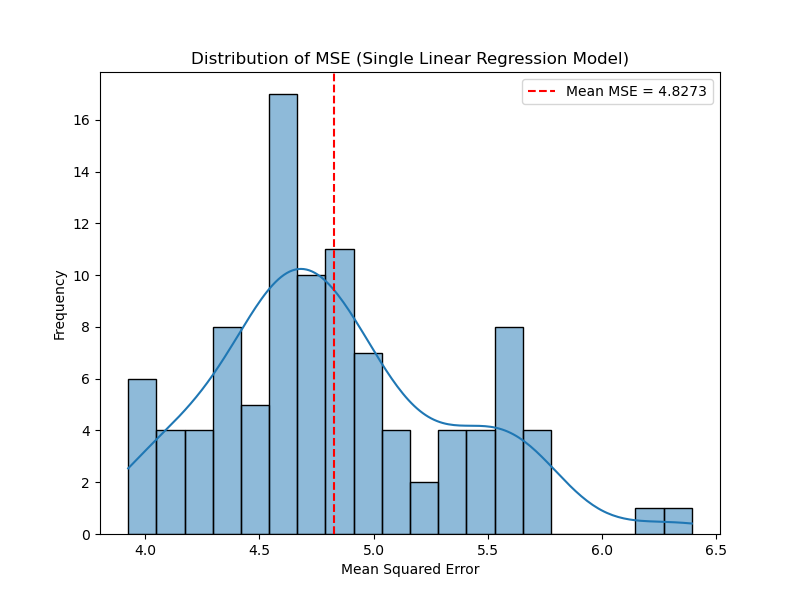
\includegraphics[width=0.45\textwidth]{./fig/Figure_1.png}
    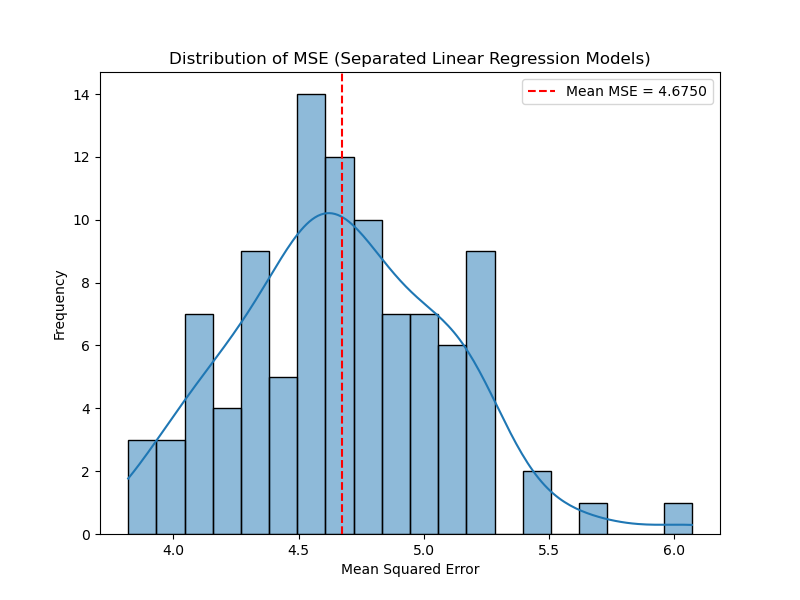
\includegraphics[width=0.45\textwidth]{./fig/Figure_2.png}
    \caption{Left: Single Linear Regression Model; Right: Gender-Separated Linear Regression Model}
    \label{fig:comparison}
\end{figure}


\begin{figure}[htbp]
    \centering
    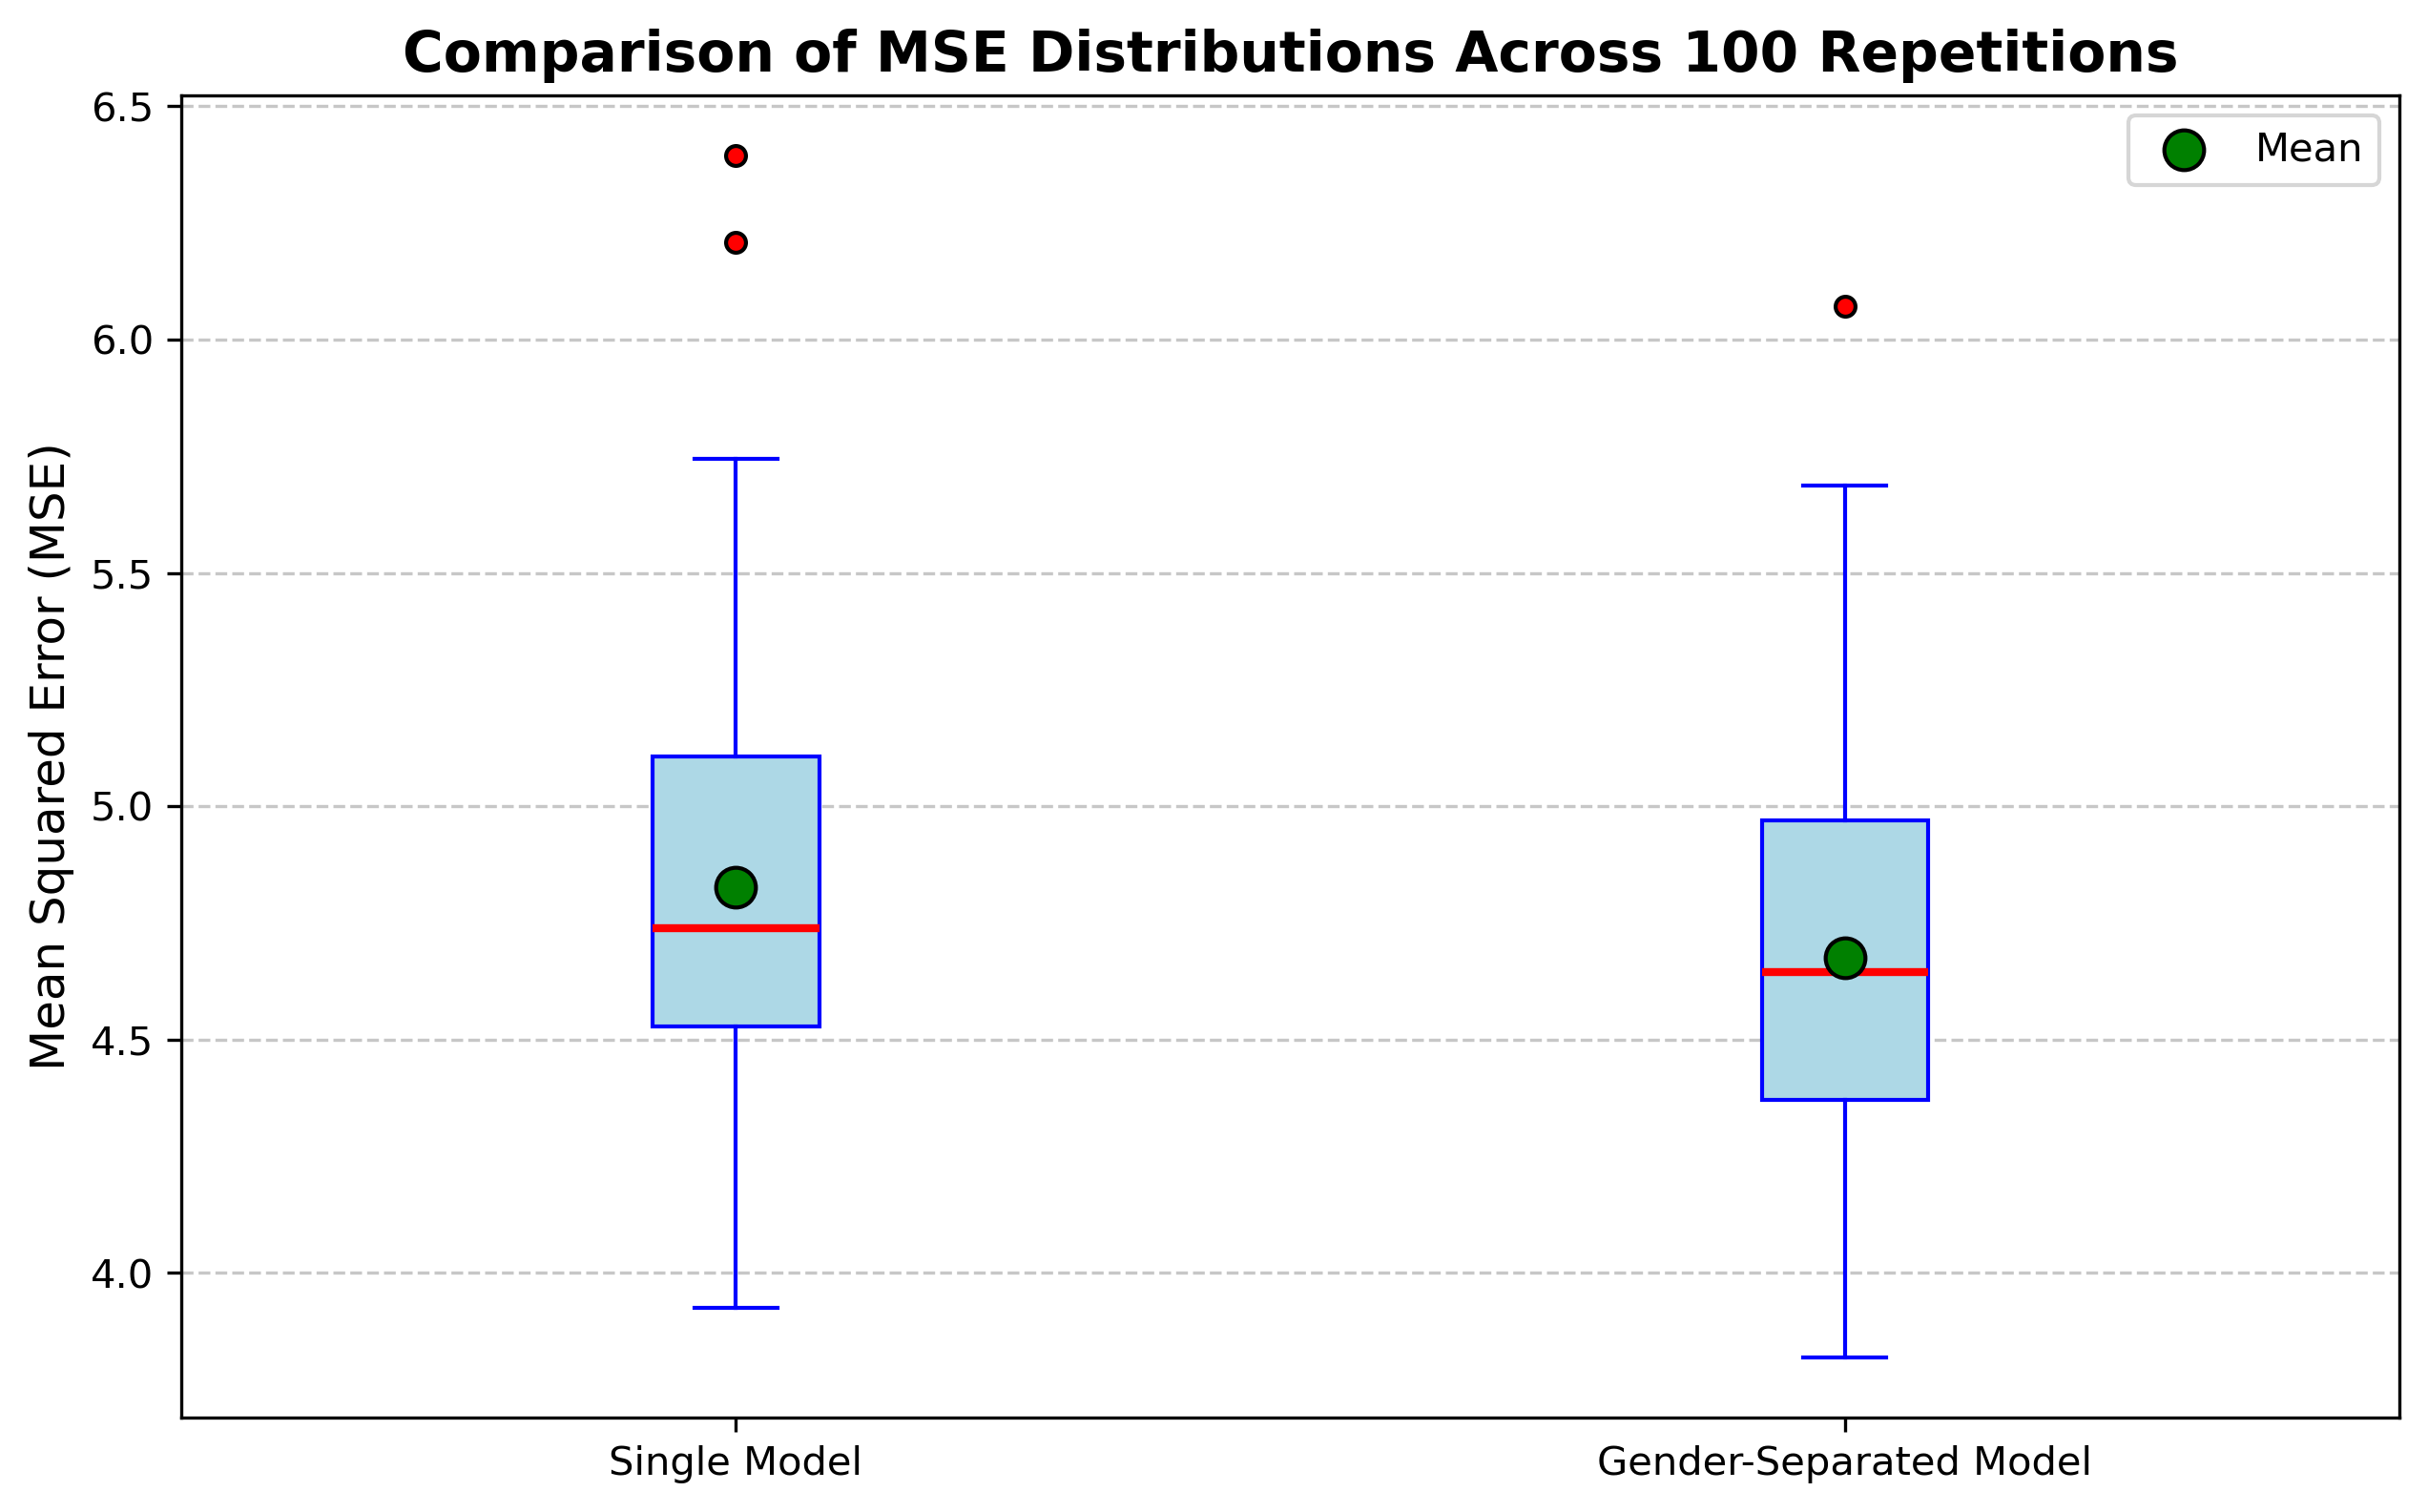
\includegraphics[width=0.8\textwidth]{./fig/MSE_comparison_boxplot.png}
    \caption{Boxplot of MSE}
    \label{fig:boxplot_mse}
\end{figure}
\end{document}